%%%% utfpr-slides.tex, 2019/12/01
%%%% Copyright (C) 2015-2019 Luiz E. M. Lima (luizeduardomlima@gmail.com)
%%
%% This work may be distributed and/or modified under the conditions of the
%% LaTeX Project Public License, either version 1.3 of this license or (at your
%% option) any later version.
%% The latest version of this license is in
%%   http://www.latex-project.org/lppl.txt
%% and version 1.3 or later is part of all distributions of LaTeX version
%% 2005/12/01 or later.
%%
%% This work has the LPPL maintenance status `maintained'.
%%
%% The Current Maintainer of this work is Luiz E. M. Lima.
%%
%% This work consists of the files utfpr-slides.sty and utfpr-slides.tex.
%%
%% A brief description of this work is in readme.txt.

%% Detecção e aviso sobre comandos obsoletos
% \RequirePackage[l2tabu, orthodox]{nag}

%% Classe de documento e opções
%%%% Modo apresentação: descomente o comando \documentclass[]{beamer}
\documentclass[%% Opções: [*] comente para remover; [>] passada para pacotes
  10pt,%% Tamanho de fonte: 10pt, 11pt, 12pt, etc.
  aspectratio = 43,%% Razão de aspecto: 169 (16:9), 43 (4:3), etc.
  compress,%% Redução de tamanho das barras de navegação [*]
  % handout,%% Versão que usa especificações de sobreposição do folheto [*]
  t,%% Alinhamento vertical dos quadros: b (fundo), c (centro) e t (topo)
  english,%% Idioma secundário (penúltimo) [>]
  brazilian,%% Idioma primário (último) [>]
]{beamer}
%%%% Modo artigo: descomente o comando \documentclass[]{article}
% \documentclass[%% Opções: [>] passada para pacotes
  % a4paper,%% Tamanho de papel: a4paper, letterpaper, etc.
  % english,%% Idioma secundário (penúltimo) [>]
  % brazilian,%% Idioma primário (último) [>]
% ]{article}

%% Pacotes utilizados
\usepackage[%% Opções:
  Times   = false,%% Fontes Times (roman) e Arial (sans serif): true ou false
  BibURLs = false,%% Links de URLs nas referências: true ou false
  GovLogo = false,%% Logomarca do Governo Federal: true ou false
  MECLogo = false,%% Logomarca do Ministério da Educação: true ou false
  LogosOn = false,%% Logomarcas nos títulos dos slides: true ou false
  ABNTNum = none,%% Estilo numérico ABNT: none (AUTOR, ANO), dflt (1) e brkt [1]
]{utfpr-slides}

\usepackage{siunitx}
\usepackage{listings}
\usepackage{color}
\usepackage[super]{nth}
\usepackage{datetime}
\beamertemplatenavigationsymbolsempty
\iflanguage{english}{%
  \newdateformat{myformat}{\monthname[\THEMONTH]  \nth{\THEDAY}, \THEYEAR}
}{
\newdateformat{myformat}{\THEDAY de \monthname[\THEMONTH] de \THEYEAR}
}
\definecolor{mylilas}{RGB}{170,55,241}
\lstset{language=Matlab,%
	basicstyle=\footnotesize\ttfamily,breaklines=true,%
	morekeywords={matlab2tikz},
	keywordstyle=\color{blue},%
	morekeywords=[2]{1}, keywordstyle=[2]{\color{black}},
	%morekeywords={laplace,ilaplace},
	deletekeywords={roots,residue,poly,polyder},
	identifierstyle=\color{black},%
	stringstyle=\color{mylilas},
	commentstyle=\color{black!50!green},%
	upquote=true,
	showstringspaces=false,%without this there will be a symbol in the places where there is a space
	%    numbers=left,%
	%    numberstyle={\tiny \color{black}},% size of the numbers
	%    numbersep=9pt, % this defines how far the numbers are from the text
	%emph=[1]{for,end,break},emphstyle=[1]\color{red}, %some words to emphasise
	%emph=[2]{word1,word2}, emphstyle=[2]{style},    
}
%% Arquivo de referências
\addbibresource{utfpr-slides.bib}

%% Arquivos de logomarcas (diretório ``Logos''): comente para remover
%\logoevent{evento}%% Logomarca do evento
%\logoorg{evento-org}%% Logomarca da organização promotora
%\logoextinst{inst-ext}%% Logomarca da instituição do autor externo
\logoprog{ppgse-ct}%% Logomarca do programa ou do curso
\logodept{ppgse-ct}%% Logomarca do departamento ou da coordenação
\logoextra{ppgse-ct}%% Logomarca extra (à esquerda da logomarca do câmpus)
\logocampus{utfpr-ct}%% Logomarca do câmpus

%% Informações do documento
%%%% Título: [CURTO]; {LONGO}
\title[Título do Trabalho Reduzido]{%
  \bfseries%
  Título do Trabalho Completo
}
%%%% Subtítulo
\subtitle{%
  Dissertação de Mestrado
}
%%%% Assunto
\subject{Nome e/ou Sigla do Congresso, Seminário ou Evento Técnico/Científico}
%%%% Congresso, seminário ou evento técnico/científico:
%%%% descomente os comandos \author[]{}, institute[]{} e \titlegraphic{}
%%%%%% Autor(es): [CURTO]; {LONGO}
\author[P. M. Autor(a) et al.]{%
  Primeiro(a)~M.~Autor(a)\inst{1}%
  \athanks[0000-0000-0000-0001]{autor1@dominio}{%
    Departamento, Coordenação, Programa ou Curso%
  }%
  \and Ohara~K.~Rayel\inst{2}%
  \athanks[0000-0002-9543-9811]{oharakr@utfpr.edu.br}{%
    Programa de Pós-Graduação em Sistemas de Energia%
  }%
  \and Terceiro(a)~M.~Autor(a)\inst{3}%
  \athanks[0000-0000-0000-0003]{autor3@dominio}{%
    Departamento, Coordenação, Programa ou Curso%
  }%
  \and\\Quarto(a)~M.~Autor(a)\inst{4}%
  \athanks[0000-0000-0000-0004]{autor4@dominio}{%
    Departamento, Coordenação, Programa ou Curso%
  }%
  \and Quinto(a)~M.~Autor(a)\inst{5}%
  \athanks[0000-0000-0000-0005]{autor5@dominio}{%
    Departamento, Coordenação, Programa ou Curso%
  }%
}
%%%%%% Instituição(ões) e e-mail(s): [CURTO]; {LONGO}
\institute[UTFPR/UFSC]{%
  \affil[1,3,5]{\utfprname, Curitiba, Paraná, Brasil}%
  \and\affil[2,4]{Universidade Federal de Santa Catarina, Florianópolis, Santa Catarina, Brasil}%
  \and\email[1]{autor1@dominio}%
  \sep\email[2]{oharakr@utfpr.edu.br}%
  \sep\email[3]{autor3@dominio}%
  \sep\email[4]{autor4@dominio}%
  \sep\email[5]{autor5@dominio}%
}
%%%%%% Logomarcas do evento
\titlegraphic{\eventlogos}
%%%% Defesa de trabalho acadêmico:
%%%% descomente os comandos \author[]{}, institute[]{} e \titlegraphic{}
%%%%%% Autor(a): [CURTO]; {LONGO}
% \author[N. Autor(a)]{%
  % Nome do(a) Autor(a)%
  % \athanks[0000-0000-0000-0000]{autor@dominio}{%
    % Departamento, Coordenação, Programa ou Curso%
  % }%
% }
%%%%%% Instituição: [CURTO]; {LONGO}
% \institute[UTFPR-PG/DEPTO/PPG]{%
  % \affil{%
    % \utfprname\ (UTFPR)%
    % \and Câmpus Ponta Grossa (PG)%
    % \and Departamento ou Coordenação (DEPTO)%
    % \and Programa ou Curso (PPG)%
  % }%
  % \and\email{autor@dominio}%
  % \and Orientador(a): Prof(a). Dr(a). Nome do(a) Orientador(a)%
% }
%%%%%% Logomarcas da instituição
% \titlegraphic{\institutelogos}
%%%% Câmpus: {SIGLA}; {NOME}
\campus{CT}{Campus Curitiba}
%%%% Departamento, coordenação, programa ou curso: [LOGO]; {SIGLA}; {NOME}
\departament[ppgse-ct]{PPGSE}{Programa de Pós-Graduação em Sistemas de Energia}
%%%% Data: [CURTO]; {LONGO}
\date[\myformat\today]{\myformat\today}

%% Início do documento
\begin{document}

\mode<presentation>{%% Modo apresentação: página de título e sumário
  \frame{\titlepage}%
%   \frame[allowframebreaks]{%
%     \frametitle{\contentsname}%
%     \framesubtitle{~}%
%     \tableofcontents%
%   }%
}

\mode<article>{\maketitle}%% Modo artigo: página de título

\section{Introdução}\label{sec:intro}

\subsection{Descrição do Documento e Formatação das Citações e Referências}\label{ssec:intro1}

\begin{frame}
Esta apresentação de slides foi desenvolvida com base na classe \href{http://www.ctan.org/pkg/beamer/}{\LaTeX/Beamer~\linkicon}.
\begin{block}{Citações e referências}
\begin{itemize}
\item Exemplos de referências podem ser observados nas citações:
\begin{itemize}
\item Implícita: \ldots\ \cite{Nriagu1988,Lamport1994,VanEkenstein1997}.
\item Explícita: Segundo \textcite{Wizentier1992,Faina2000},\ldots
\end{itemize}
\item Citações e referências podem ser inseridas neste documento usando os comandos do pacote \LaTeX\ \enquote{\href{http://ctan.org/pkg/biblatex/}{biblatex~\linkicon}}.
\item Os dados de cada referência podem ser obtidos de um arquivo \enquote{bibtex} (*.bib), geralmente na própria página de \textit{download} da referência (artigos, livros, etc.), ou no Google Acadêmico, etc.
\item Para gerar ou editar entradas de arquivos \enquote{bibtex} (*.bib), pode-se utilizar a ferramenta \enquote{\href{http://truben.no/latex/bibtex/}{Bibtex Editor~\linkicon}} ou \enquote{\href{http://zbib.org/}{ZoteroBib~\linkicon}}, entre outras.
\end{itemize}
\end{block}
\end{frame}

\section{Revisão da Literatura}\label{sec:revlit}

\subsection{Listas de Itens, com e sem Numeração}\label{ssec:revlit1}

\begin{frame}
\begin{block}<+->{Exemplo de lista de itens}
\begin{itemize}
\item Item a.
\item Item b.
\item Item c.
\end{itemize}
\end{block}
\begin{block}<+->{Exemplo de lista de itens numerados}
\begin{enumerate}[<+-|alert@+>]
\item Item numerado 1.
\begin{enumerate}[a]
\item Subitem numerado a.
\item Subitem numerado b.
\end{enumerate}
\item Item numerado 2.
\item Item numerado 3.
\end{enumerate}
\end{block}
\end{frame}

\subsection{Equações, com e sem Numeração}\label{ssec:revlit2}

\begin{frame}[fragile = singleslide]
Uma equação como $y = a x^2 + b x + c$ pode ser inserida ao longo do texto de um parágrafo usando o ambiente \LaTeX\ \enquote{math} (\verb|$...$|).
Por outro lado, a seguinte equação é um exemplo de equação não numerada inserida numa linha em separado usando o ambiente \LaTeX\ \enquote{displaymath} (\verb|\[...\]|).
\begin{block}{}
\[
\frac{\mathrm{d} y}{\mathrm{d} x} = \gamma \operatorname{sen} x
\]
\end{block}
A Eq.~\eqref{eq:fx} é um exemplo de equação inserida usando o ambiente \LaTeX\ \enquote{equation} e numerada automaticamente.
\begin{block}{}
\begin{equation}\label{eq:fx}
f(x) = \frac{1}{\alpha} \int_0^L \left(\frac{x^2}{2} - \frac{x^3}{3}\right) \mathrm{d} x
\end{equation}
\end{block}
Para gerar ou editar equações em \LaTeX, pode-se utilizar a ferramenta \enquote{\href{http://formulasheet.com/}{Formula Sheet~\linkicon}}, entre outras.
\end{frame}

\section{Material e Métodos}\label{sec:matmet}

\subsection{Figuras, e Atalhos para Arquivos (Externos)}\label{ssec:matmet1}

\begin{frame}
\begin{columns}[T]
\column{0.5\textwidth}
A Fig.~\ref{fig:campuspontagrossa} é um exemplo de figura inserida usando o ambiente \LaTeX\ \enquote{figure} e numerada automaticamente.
\begin{figure}[!htb]
\centering%
\caption{Câmpus Ponta Grossa da UTFPR.}%
\label{fig:campuspontagrossa}
\mode<presentation>{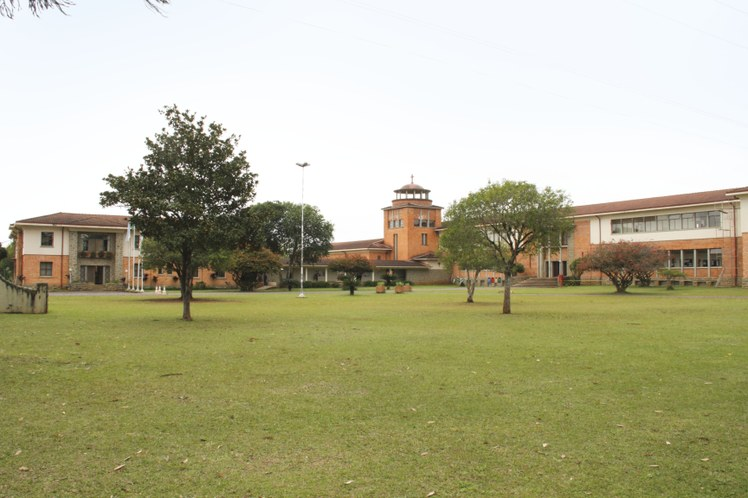
\includegraphics[width = 0.8\columnwidth]{./Figuras/campuspontagrossa}}%% Modo apresentação: tamanho da figura
\mode<article>{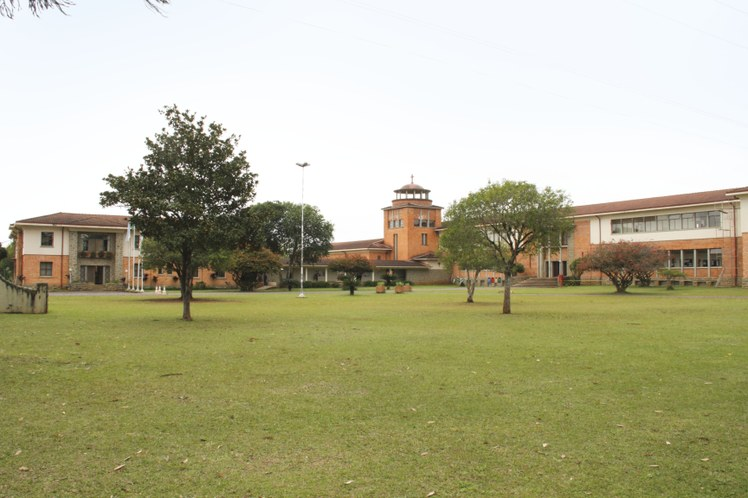
\includegraphics[width = 0.4\columnwidth]{./Figuras/campuspontagrossa}}%% Modo artigo: tamanho da figura
\source{\textcite{UTFPR2018}.}
\end{figure}
\column{0.5\textwidth}
\mode<article>{\par}%% Modo artigo: quebra de parágrafo
Atalhos para execução de arquivos (externos) também podem ser inseridos, conforme exemplo na sequência.
\begin{block}{Exemplo de atalho para vídeo}
\linktofile{./Videos/experimentofluido.flv}{Experimento de mecânica dos fluidos (vídeo).}
\href{http://tex.stackexchange.com/q/20800/5701}{\beamergotobutton{Link}}
\end{block}
\begin{block}{Exemplo de {\it link} para {\it sites}}
\href{http://www.ppgse.ct.utfpr.edu.br}{\beamergotobutton{Site do PPGSE}}
\end{block}
\end{columns}
\end{frame}

\subsection{Tabelas, e Informações e Dicas sobre \TeX/\LaTeX}\label{ssec:matmet2}

\begin{frame}
\begin{columns}[T]
\column{0.5\textwidth}
A Tab.~\ref{tab:Ldimens} é um exemplo de tabela inserida usando o ambiente \LaTeX\ \enquote{table} e numerada automaticamente.
\begin{table}[!htb]
\centering%
\mode<presentation>{\scriptsize}%% Modo apresentação: tamanho de fonte
\mode<article>{\small}%% Modo artigo: tamanho de fonte
\caption{Exemplo de legenda de tabela.}%
\label{tab:Ldimens}
\begin{tabular*}{\columnwidth}{@{\extracolsep{\fill}}llll}
\toprule
$L$   & $L^2$     & $L^3$     & $L^4$     \\
{[\si{\meter}]} & {[\si{\meter}$^2$]} & {[\si{\meter}$^3$]} & {[\si{\meter}$^4$]} \\
\midrule
1     & 1         & 1         & 1         \\
2     & 4         & 8         & 16        \\
3     & 9         & 27        & 81        \\
4     & 16        & 64        & 256       \\
5     & 25        & 125       & 625       \\
\bottomrule
\addlinespace
\end{tabular*}
\source{autoria própria.}
\end{table}
\mode<article>{\par}%% Modo artigo: quebra de parágrafo
Para gerar ou editar tabelas em \LaTeX, pode-se utilizar a ferramenta \enquote{\href{http://www.tablesgenerator.com/}{Tables Generator~\linkicon}}, entre outras.
\column{0.5\textwidth}
\begin{block}{Informações e dicas sobre \TeX/\LaTeX}
\begin{itemize}
\item \href{http://www.latex-project.org/}{\LaTeX\ Project~\linkicon}.
\item \href{http://www.ctan.org/}{Comprehensive \TeX\ Archive Network (CTAN)~\linkicon}.
\item \href{http://www.tug.org/}{\TeX\ Users Group (TUG)~\linkicon}.
\item \href{http://en.wikibooks.org/wiki/LaTeX/}{\LaTeX\ --- Wikibooks~\linkicon}.
\item \href{http://tex.stackexchange.com/}{\TeX-\LaTeX\ Stack Exchange~\linkicon}.
\end{itemize}
\end{block}
\end{columns}
\end{frame}

\section{Resultados e Discussão}\label{sec:resuldisc}

\subsection{Mais Exemplos de Figuras}\label{ssec:resuldisc1}

\begin{frame}[allowframebreaks]
As Figs.~\ref{fig:graficoxy1} e~\ref{fig:graficoxy2} são mais exemplos de figuras inseridas usando o ambiente \LaTeX\ \enquote{figure} e dispostas em duas colunas.
\begin{columns}[T]
\column{0.5\textwidth}
\begin{figure}[!htb]
\centering%
\caption{Exemplo de legenda de figura.}%
\label{fig:graficoxy1}
\mode<presentation>{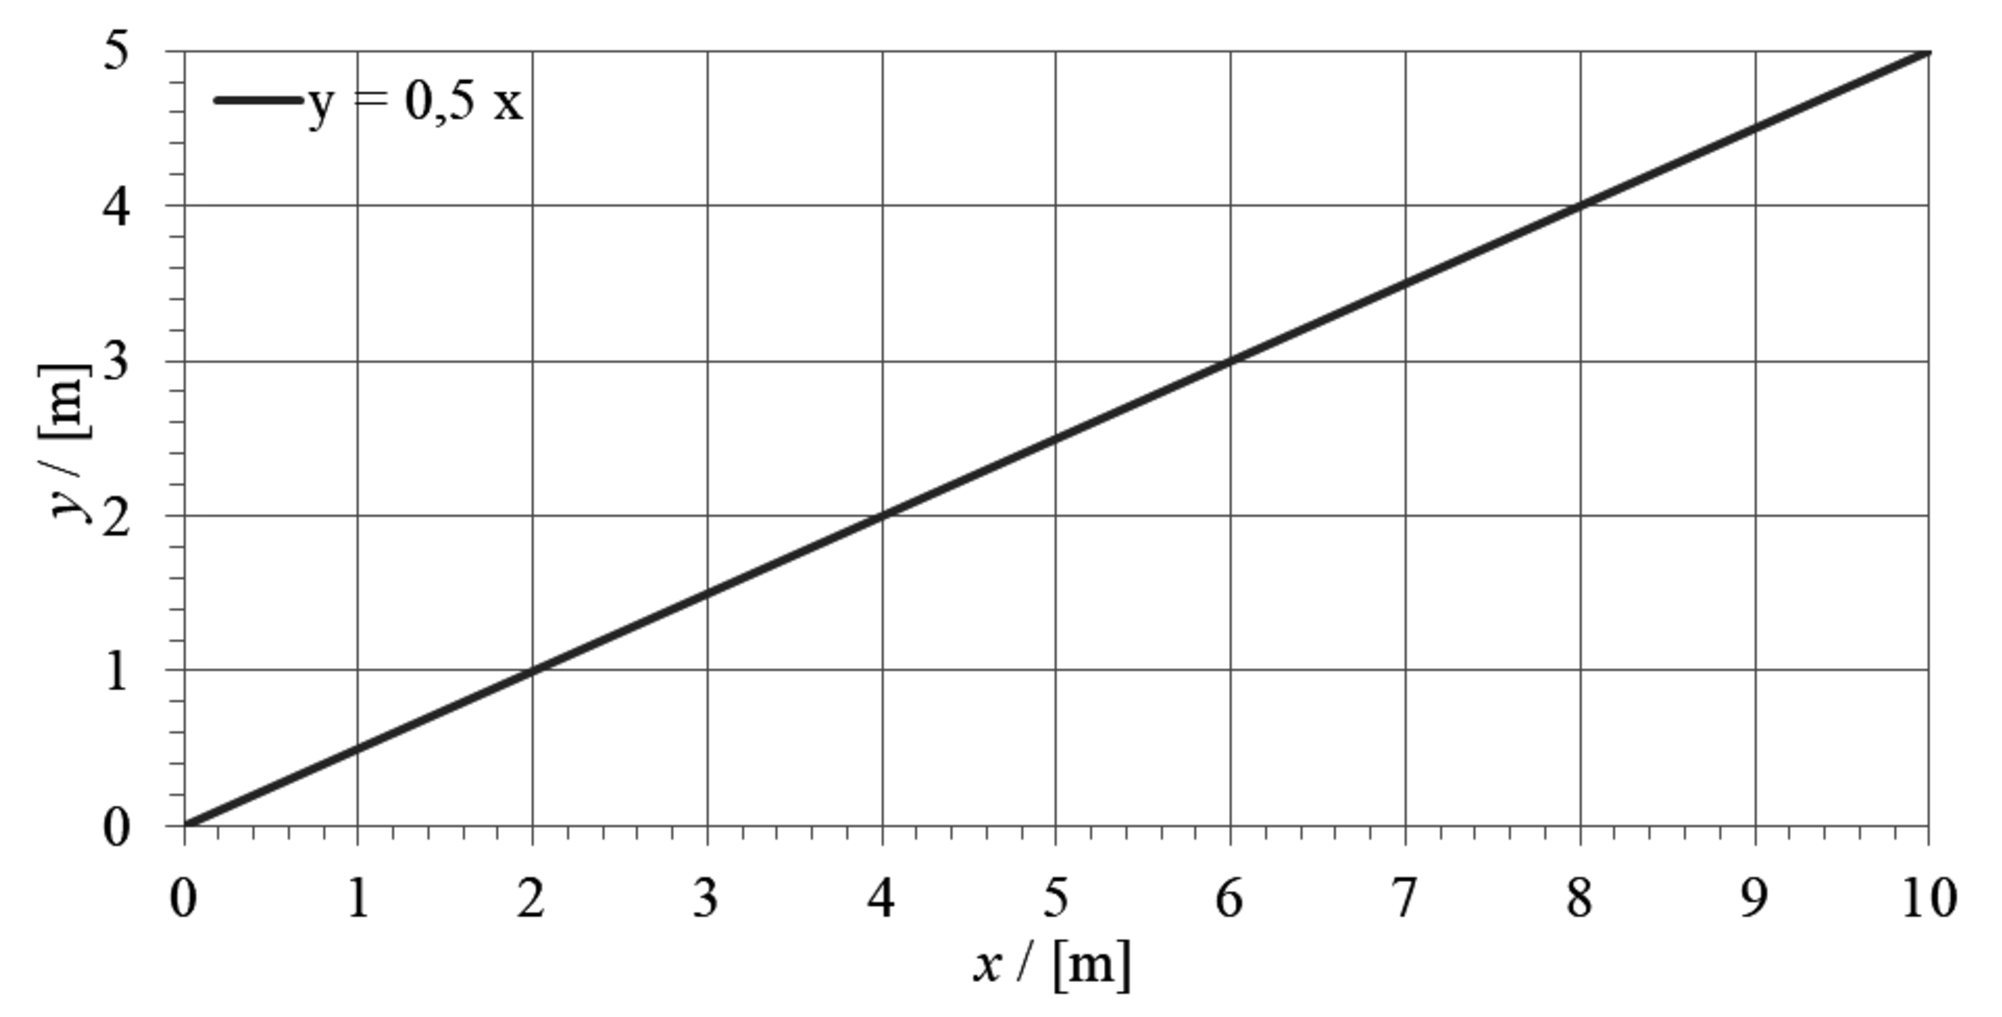
\includegraphics[width = \columnwidth]{./Figuras/graficoxy}}%% Modo apresentação: tamanho da figura
\mode<article>{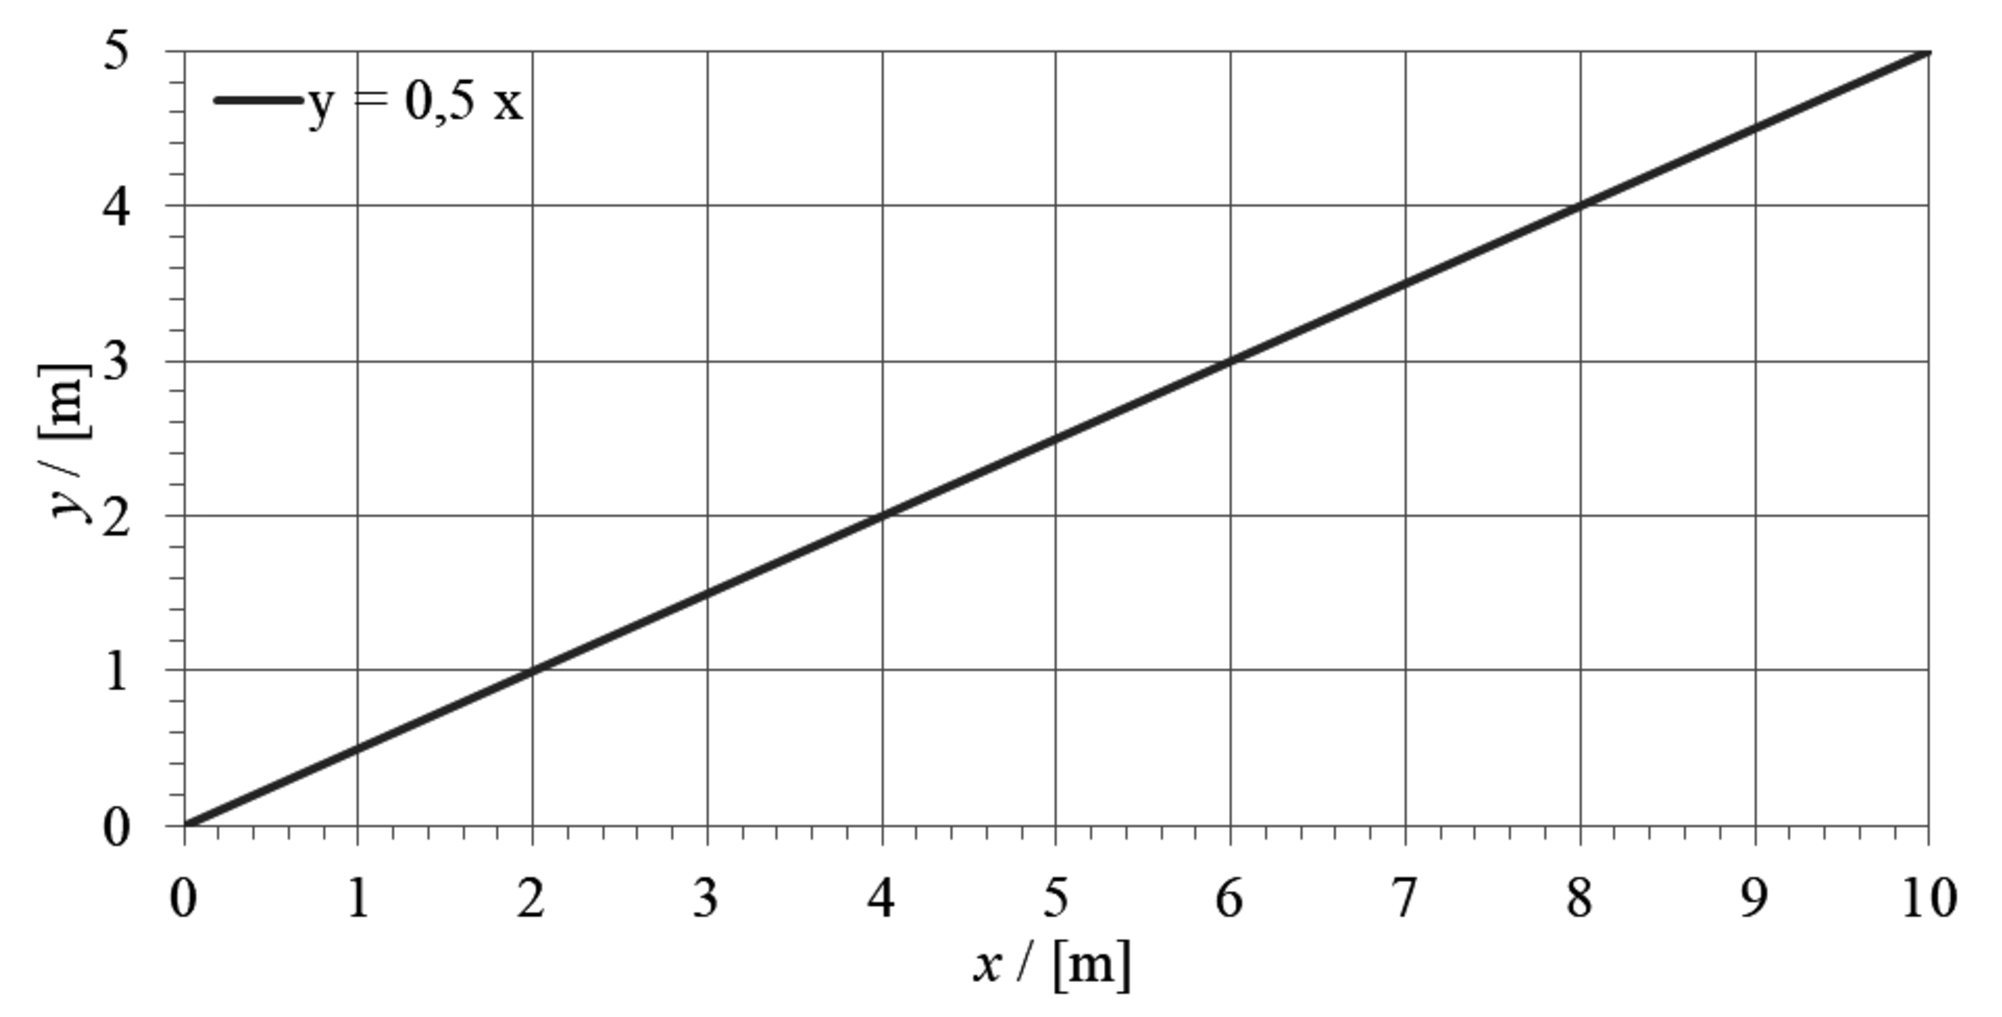
\includegraphics[width = 0.5\columnwidth]{./Figuras/graficoxy}}%% Modo artigo: tamanho da figura
\source{autoria própria.}
\end{figure}
\column{0.5\textwidth}
\begin{figure}[!htb]
\centering%
\caption{Exemplo de legenda de figura.}%
\label{fig:graficoxy2}
\mode<presentation>{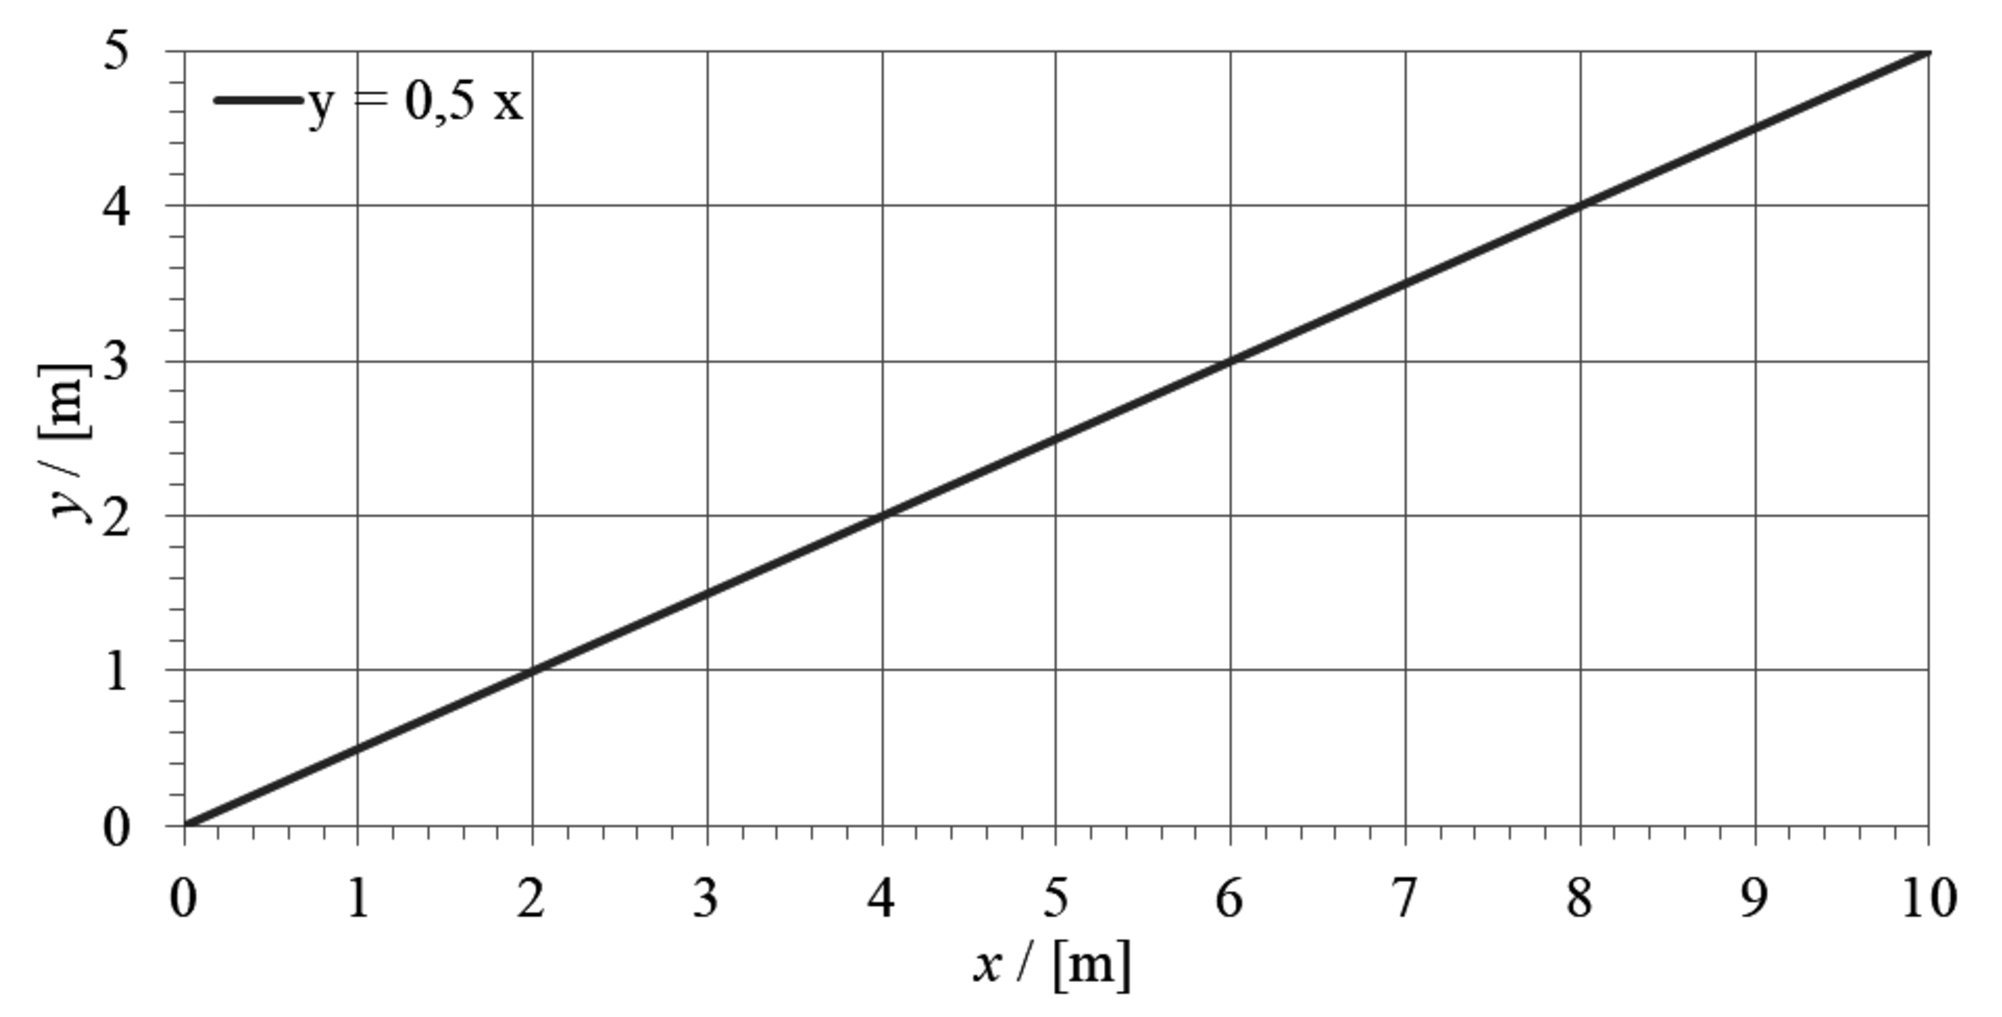
\includegraphics[width = \columnwidth]{./Figuras/graficoxy}}%% Modo apresentação: tamanho da figura
\mode<article>{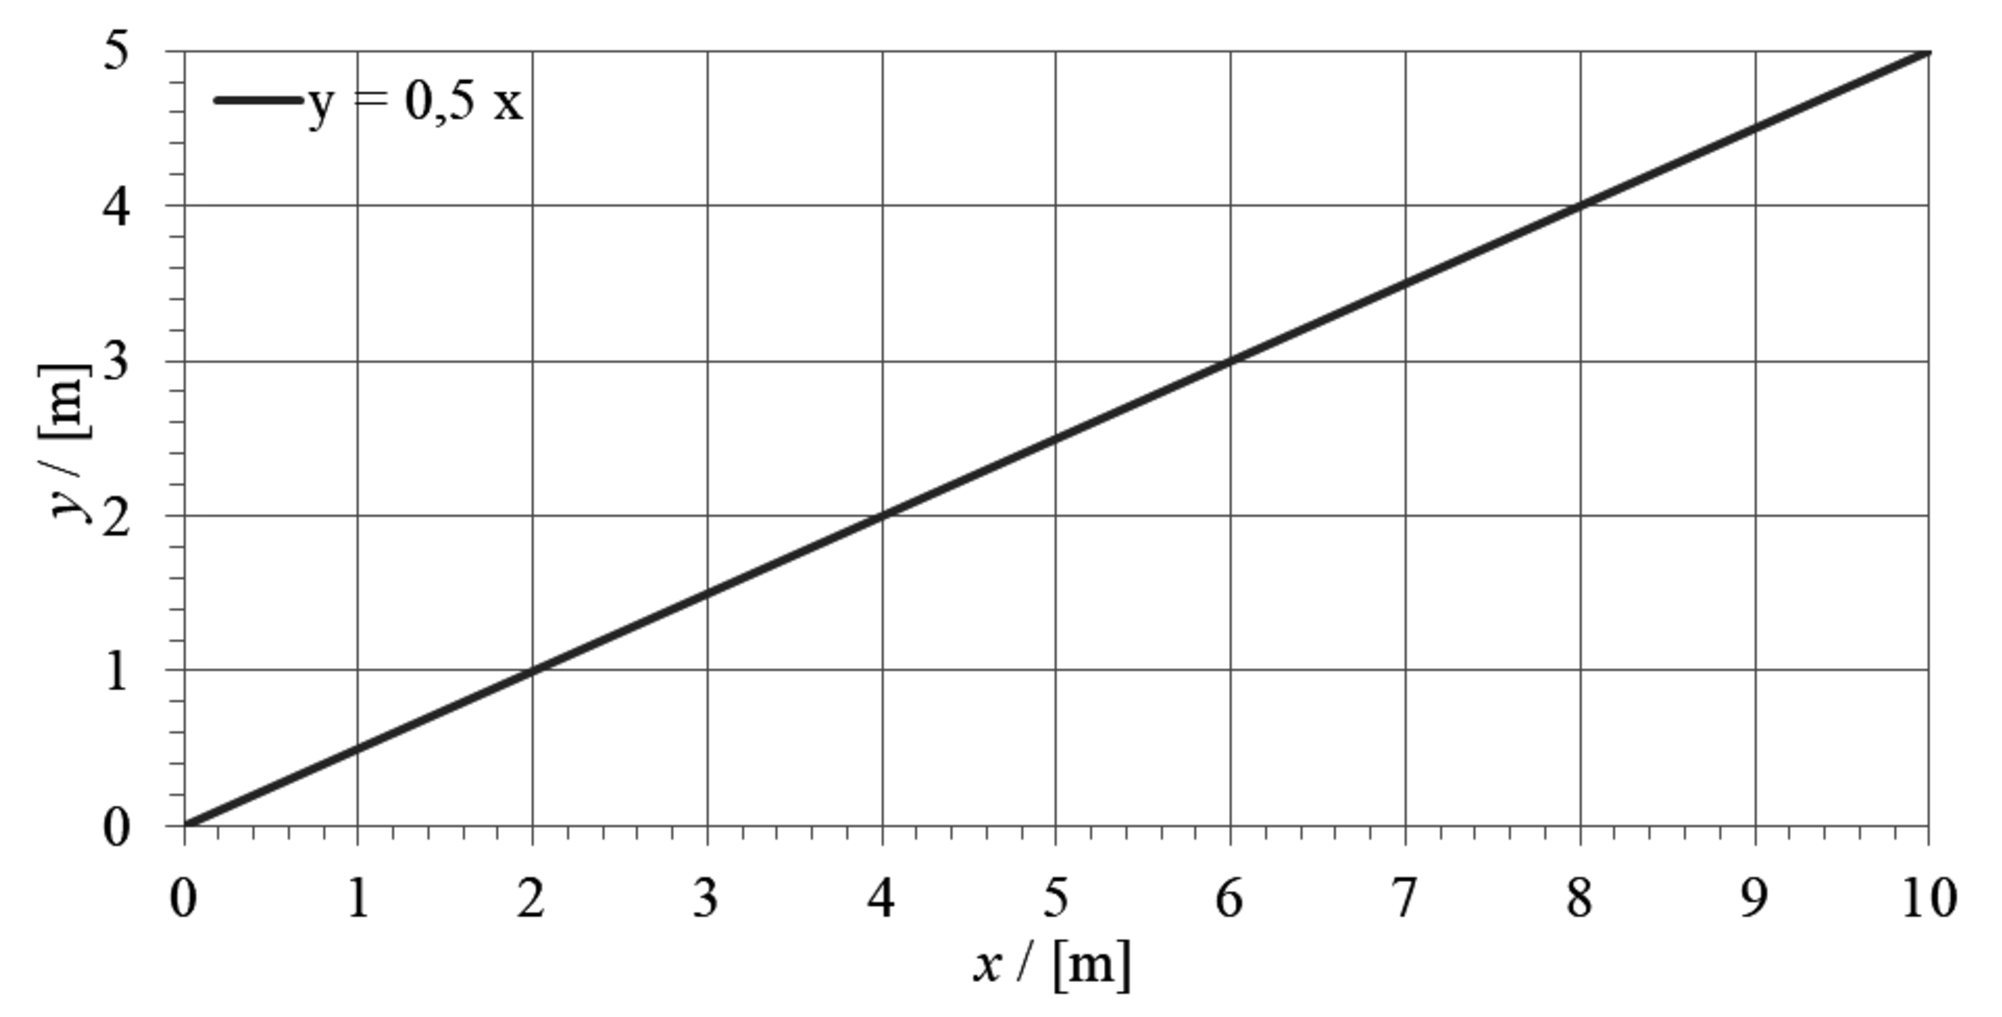
\includegraphics[width = 0.5\columnwidth]{./Figuras/graficoxy}}%% Modo artigo: tamanho da figura
\source{autoria própria.}
\end{figure}
\end{columns}
\framebreak%
\mode<article>{\par}%% Modo artigo: quebra de parágrafo
A Fig.~\ref{fig:mapacampus} apresenta um mapa com a localização dos câmpus da UTFPR\@.
\begin{figure}[!htb]
\centering%
\caption{Mapa com a localização dos câmpus da UTFPR.}%
\label{fig:mapacampus}
\mode<presentation>{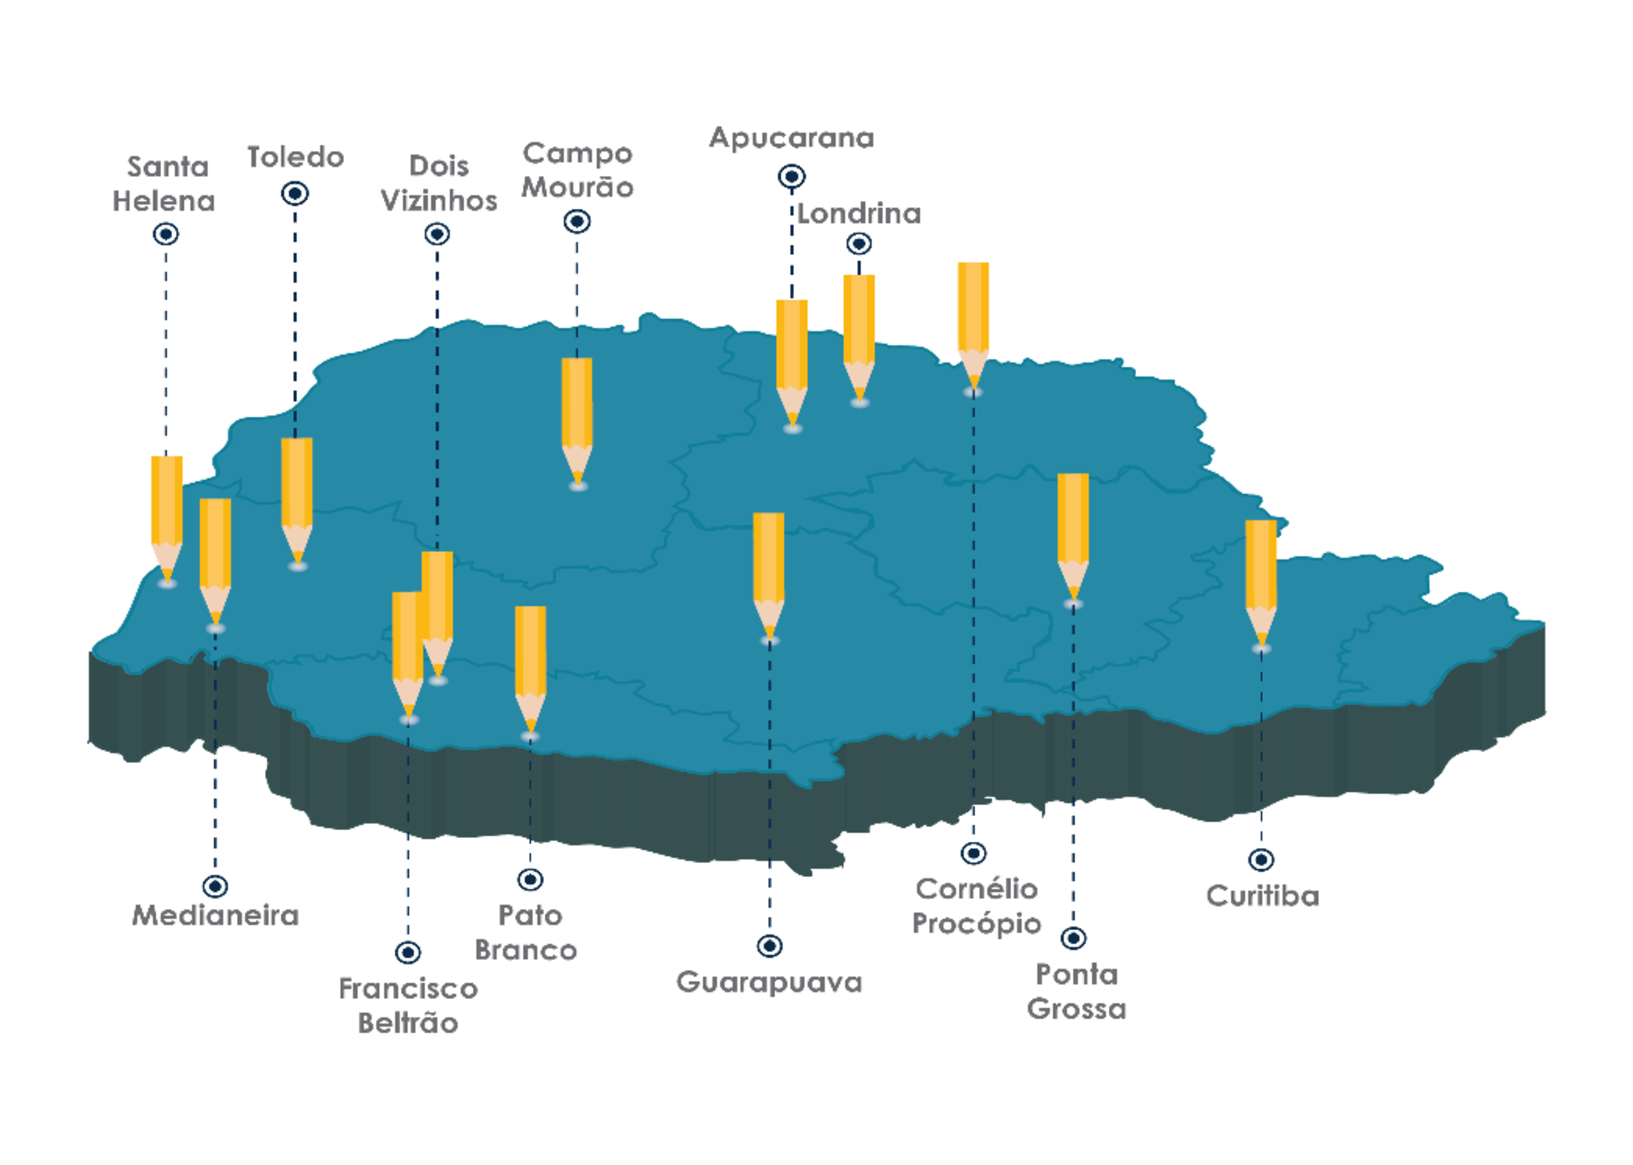
\includegraphics[width = 0.4\columnwidth]{./Figuras/mapacampus}}%% Modo apresentação: tamanho da figura
\mode<article>{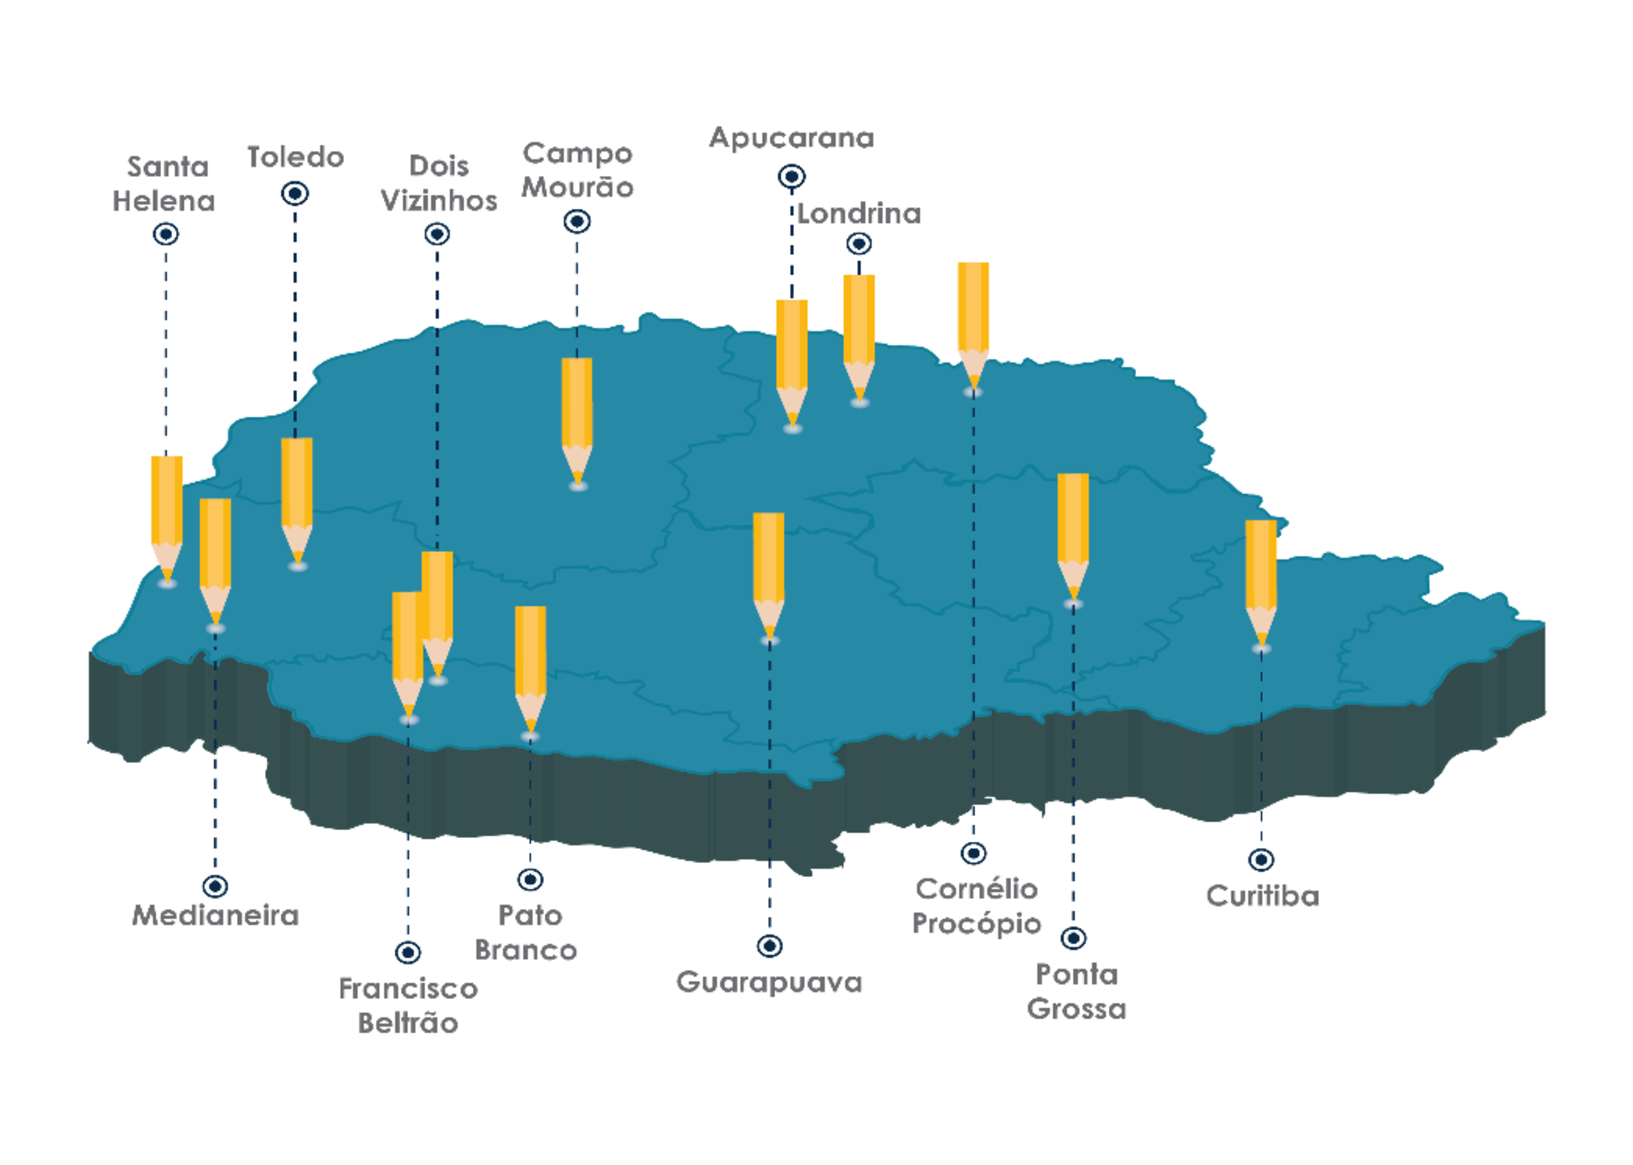
\includegraphics[width = 0.2\columnwidth]{./Figuras/mapacampus}}%% Modo apresentação: tamanho da figura
\source{\textcite{UTFPR2018}.}
\end{figure}
\end{frame}


\begin{frame} {Figura com Transparência}

\begin{columns}
\column{8cm}
\begin{figure}[!htb]
\centering%
%\caption{Exemplo de legenda de figura.}%
\label{fig:cdf}
\mode<presentation>{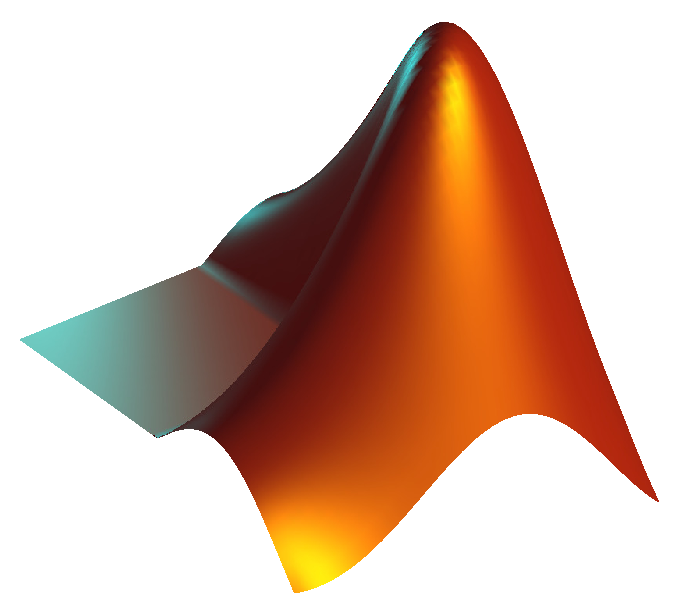
\includegraphics[width = 0.9\columnwidth]{./Figuras/test.eps}}%% Modo apresentação: tamanho da figura
%\source{autoria própria.}
\end{figure}
\column{4cm}
\begin{itemize}
\vfill
\item \url{https://github.com/altmany/export_fig}
\vfill
\item \lstinline{set(gca, 'Color', 'none');}
\vfill
\item \lstinline{export_fig nomedasuafigura.eps -transparent}
\vfill
\end{itemize}
\end{columns}

\end{frame}

\section{Conclusões}\label{sec:concl}

\subsection{Descrição das Conclusões Obtidas}\label{ssec:concl1}

\begin{frame}
\begin{block}{Lista de conclusões}
\begin{itemize}
\item Conclusão 1.
\item Conclusão 2.
\item Conclusão 3.
\item Conclusão 4.
\item Conclusão 5.
\end{itemize}
\end{block}
\end{frame}

\mode<presentation>{%% Modo apresentação: referências
  \section{\refname}\label{sec:refs}%
  \frame[allowframebreaks]{%
    \framesubtitle{~}%
    \printbibliography[heading = none]%
  }%
}

\mode<article>{\printbibliography}%% Modo artigo: referências

\section{Agradecimentos}\label{sec:agrad}

\respnotice[Declaração de Responsabilidade]{O(s) autor(es) é(são) o(s) único(s) responsável(eis) pelas informações contidas neste documento.}

\begin{frame}{}{\mode<presentation>{~}}
Às organizações de fomento, pelo apoio recebido para o desenvolvimento deste trabalho e a participação neste evento:
\begin{center}

\includegraphics[height = 10mm]{./Logos/apoio-capes}
\hfill%

\includegraphics[height = 10mm]{./Logos/apoio-cnpq}
\hfill%

\includegraphics[height = 10mm]{./Logos/apoio-fa-gov-pr}
\hfill%

\includegraphics[height = 10mm]{./Logos/utfpr}
\end{center}
\mode<presentation>{%% Modo apresentação: agradecimentos e declaração de responsabilidade
  Aos presentes, pela atenção\sfootnote[frame]{\faStickyNoteO~\textbf{\respnoticetitle:}\space\MakeLowercase{\respnoticetext}}.%
}
\end{frame}

\mode<article>{%% Modo artigo: declaração de responsabilidade
  \section{\respnoticetitle}\label{sec:declar}%
  \respnoticetext%
}

%% Fim do documento
\end{document}
